\begin{document}
%%%%%%%%%%%%%%%%%%%%%%%%%%%%%%%%%%%%%%%%%%%%%%%%%%%%%%%%%%%%%%%%%%%%%%
\section{消火用機構}
消火方法は前述の通りであるが,ここではそのための機構であるアーム機構について述べる.

\subsection{往復スライダ・クランク機構}
アームは垂直方向に上下する1リンク機構を考える.これは,消火方法がストッパを外すという単純なものであるからだ.

アームの動作には,往復スライダ・クランク機構を採用する(図\ref{arm_con}).これは,回転運動を直線運動に変換する機構であり,回転はローテーションモータ「GWS S35 STD」から得る.クランク腕長さを$r$,連接棒長さを$l$とするとその理想的なリンク比$\rho$は,

\begin{equation}
	\rho = \frac{r}{l}=\frac{1}{3}
\end{equation}
とされている.今回は,必要なストローク長が$80$[mm]であったのでそれぞれ,$r=20$[mm],$l=60$[mm]とした.実際に製作したアームを図.\ref{arm_real}に示す.

\begin{figure}[h]
 \centering
   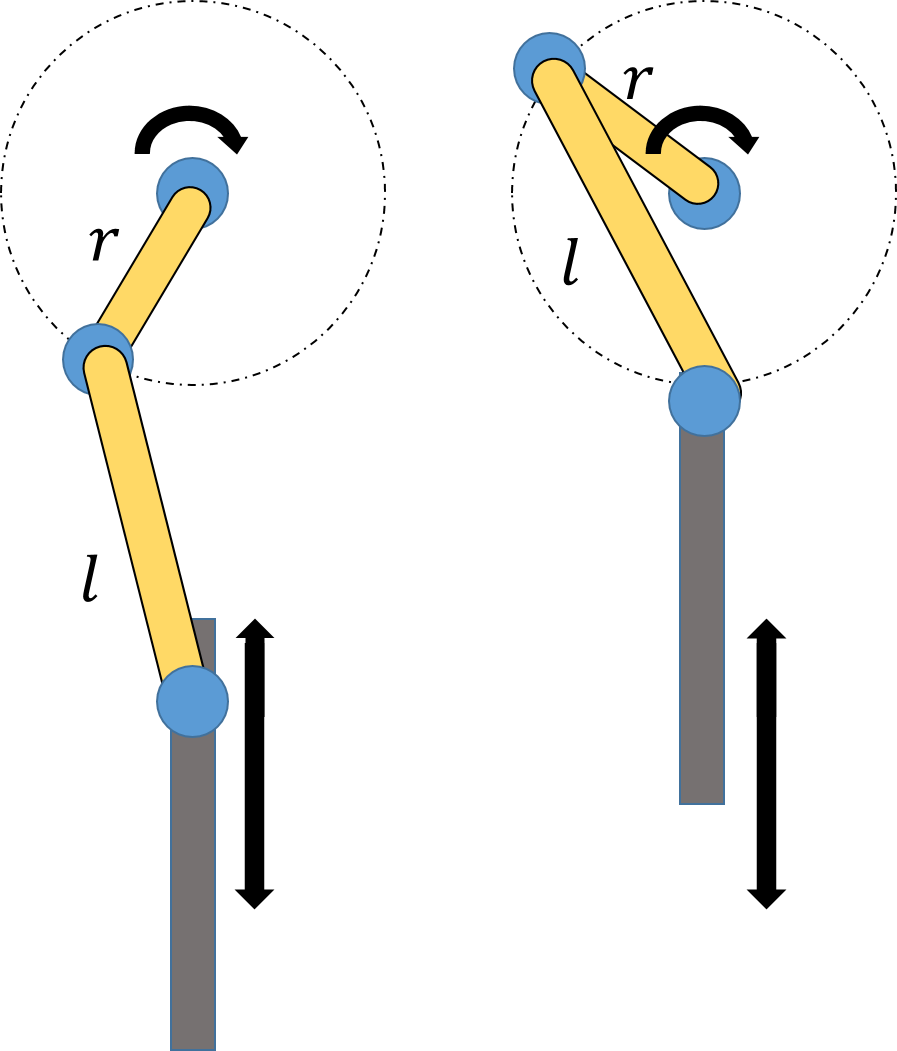
\includegraphics[clip,scale=0.3]{../kakeru_last/picture/slide_clank.png}
   \caption{消火用アーム概念図}
 \label{arm_con}
\end{figure}

\begin{figure}[h]
 \centering
 \begin{tabular}{c}

  \begin{minipage}{0.3\hsize}
   \centering
   \includegraphics[clip,scale=0.06]{../kakeru_last/picture/arm_left.png}
   \hspace{1.6cm} [1]アーム 左
  \end{minipage}
  
  \begin{minipage}{0.45\hsize}
   \centering
   \includegraphics[clip,scale=0.06]{../kakeru_last/picture/arm_right.png}
   \hspace{1.6cm} [2]アーム 右
  \end{minipage}
 \end{tabular}
 \caption{消火用アーム}
 \label{arm_real}
\end{figure}

\newpage
\subsection{使用モータ}
ローテーションモータ(図\ref{servo})の使用について示す.

[GWS S35 STD]
\begin{itemize}
 \item トルク        : 4.1 [kg] (@4.8 [V])
 \item スピード      : 0.27 [sec]/60[deg] (@4.8 [V])
 \item 重量          : 41 [g]
 \item サイズ        :$39.5 \times 20 \times 35.6$[mm]
\end{itemize}

\begin{figure}[h]
  \centering
    \includegraphics[clip,scale=0.05]{../kakeru_last/picture/servo.png}
    \caption{ローテーションモータ [ GWS S35 SSTD ]}
  \label{servo}
\end{figure}

%%%%%%%%%%%%%%%%%%%%%%%%%%%%%%%%%%%%%%%%%%%%%%%%%%%%%%%%%%%%%%%%%%%%%%%%%%%%
\end{document}